%\chapter{\Objectiveonename}
\chapter{Theorical Background Attention Mechanisms and Transformer Architectures} \label{ch:chapter_2}

\subsection{Attention Mechanisms}

In recent years, models based on Transformer architectures have revolutionized the field of natural language processing, computer vision, and other machine learning tasks. At the core of these architectures lie attention mechanisms, a powerful technique that has demonstrated its effectiveness in capturing long-range relationships and dependencies between elements in a sequence of data, allowing the model to focus primarily on the relevant parts of the input data when solving a task. This section focuses on the theory behind attention mechanisms, highlighting their relevance in the Transformer architecture and their fundamental role in enabling these models to comprehend complex contexts and generate high-quality representations. Throughout this chapter, we will explore in detail how attention mechanisms enable Transformers to overcome the limitations of traditional architectures, paving the way for a new paradigm in natural language processing, computer vision, and deep learning in general.

\newpage

\begin{figure}[h!]
    \centering%width=0.7\linewidth
    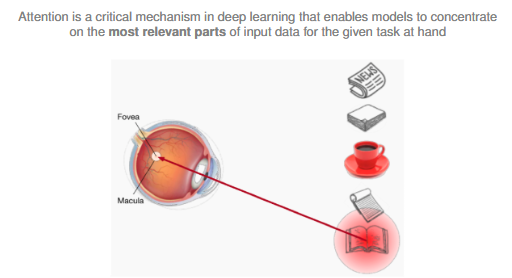
\includegraphics[width=\linewidth]{Figures/background/Attention_Mechanisms_Importance.png}
    \caption{Attention Mechanisms Importance, (\cite{goodfellow2016dive})}
    \label{fig:attention}
\end{figure}


\textbf{Queries, Keys and Values}
\\\\
For a model to primarily focus on the relevant parts of the input data when solving a task through attention mechanisms, it is essential to project the input data into different subspaces of representation. This enables the exchange of information and the capture of relationships, thereby allowing the model to assign attention weights to the input data. By doing so, the model can concentrate on the most relevant elements and establish significant dependencies between the data. 

The input $\mathbf{X}$ is transformed into the query matrix $\mathbf{Q}$, the key matrix $\mathbf{K}$, and the value
matrix $\mathbf{K}$ via three linear transformations:

\begin{equation}
    \mathbf{Q}=\mathbf{X}\mathbf{W_{Q}}
\end{equation}

\begin{equation}
    \mathbf{K}=\mathbf{X}\mathbf{W_{K}}
\end{equation}

\begin{equation}
    \mathbf{V}=\mathbf{X}\mathbf{W_{V}}
\end{equation}

where $\mathbf{W_{Q}} \in \mathbb{R}^{d \times d_{k}}$, $\mathbf{W_{K}} \in \mathbb{R}^{d \times d_{k}}$ and $\mathbf{W_{V}} \in \mathbb{R}^{d \times d_{v}}$ are parameters learnable by the model (\textbf{Backpropagation}).

\begin{figure}[h!]
    \centering%width=0.7\linewidth
    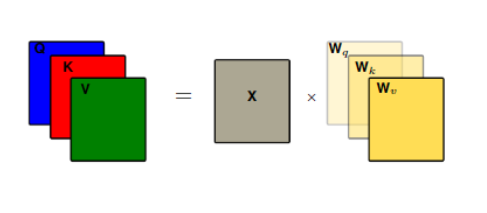
\includegraphics[width=\linewidth]{Figures/background/Linear_Transformations (1).png}
    \caption{Queries, Keys and Values Matrix, (\cite{goodfellow2016dive})}
    \label{fig:attention}
\end{figure}


\textbf{Attention Pooling Operation}
\\\\
From the concept of a database, we can establish an analogy to understand how attention mechanisms work in capturing relevant information. Let's consider a database $\mathbf{D}$ of $m$ tuples of keys and values as the representation of our input data.

\begin{equation}
    \mathbf{D}={(\mathbf{k_1},\mathbf{v_1}),...,(\mathbf{k_m},\mathbf{v_m})}
\end{equation}

and $\mathbf{q}$ is a query that we do on the database, we can define the attention of $\mathbf{q}$ on $\mathbf{D}$ throught the \textbf{attention pooling operation}:

\newpage

\begin{figure}[h!]
    \centering%width=0.7\linewidth
    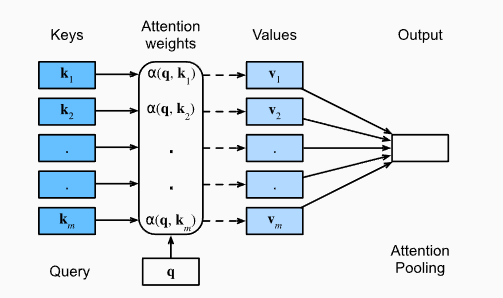
\includegraphics[width=\linewidth]{Figures/background/attention_pooling.png}
    \caption{The attention mechanism computes a linear combination over values $\mathbf{v_{i}}$ via attention pooling, where weights are derived according to the compatibility between a query $\mathbf{q}$ and keys $\mathbf{k_{i}}$, (\cite{goodfellow2016dive})}
    \label{fig:attention}
\end{figure}


\begin{equation}
    Attention(\mathbf{q},\mathbf{D})=\sum_{i=1}^{m} \alpha (\mathbf{q},\mathbf{k_i})\mathbf{v_{i}} \in \mathbb{R}^{d_{v}}
\end{equation}

where:

\begin{itemize}
    \item $\mathbf{q} \in \mathbb{R}^{d_k}$
    \item $\mathbf{k_{i}} \in \mathbb{R}^{d_k}$               
    \item $\mathbf{v_{i}} \in \mathbb{R}^{d_v}$
    \item $\alpha (\mathbf{q},\mathbf{k_{i}}) \in \mathbb{R}(i=1,...,m)$ is the attention weights or the attention function
\end{itemize}

Then de attention mechanism will attend more to the values to the which the attention weight.


\newpage


\textbf{Attention Scoring Function}

In this section we will see how to calculate the attention weights:

\begin{figure}[h!]
    \centering%width=0.7\linewidth
    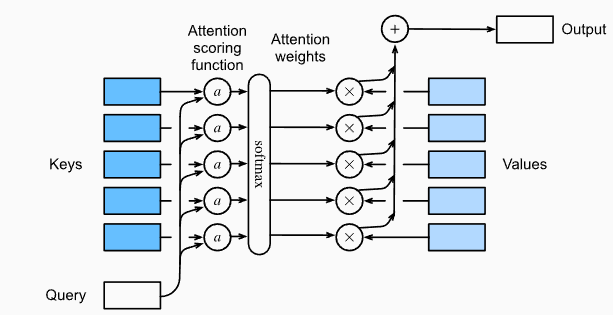
\includegraphics[width=\linewidth]{Figures/background/attention_pooling_softmax.png}
    \caption{Computing the output of attention pooling as a weighted average of values, where weights are computed with the attention scoring function 
 and the softmax operation, (\cite{goodfellow2016dive})}
    \label{fig:attention}
\end{figure}



The following are some attention functions:

\begin{itemize}
    \item Gaussian Attention Function:
    \begin{equation}  
    \alpha (\mathbf{q},\mathbf{k_{i}})=exp(-\frac{1}{2}\lVert \mathbf{q}-\mathbf{k_{i}} \rVert_2^{2}) \in \mathbb{R}
    \end{equation}
    
    \item Boxcar Attention Function:
    \begin{equation}
    \alpha (\mathbf{q},\mathbf{k_{i}})=1 \text{ if } \lVert \mathbf{q}-\mathbf{k_{i}} \rVert_2 \leq 1 \in \mathbb{R}
    \end{equation}

    
    \item Epanechikov Attention Function:
    \begin{equation}
    \alpha (\mathbf{q},\mathbf{k_{i}})=max(0,1-\lVert \mathbf{q}-\mathbf{k_{i}} \rVert_2) \in \mathbb{R}
    \end{equation}
\end{itemize}

\newpage

\textbf{Dot Product Attention Function}
Previous attention Functions are not used in transformer architectures, but the \textbf{Dot Product Attention Function} is a very used attention function used in transformer architectures. Let's start from the gaussian attention function without exponentiation (To reduce computational cost):

\begin{equation}
    \alpha (\mathbf{q},\mathbf{k_{i}})=-\frac{1}{2}\lVert \mathbf{q}-\mathbf{k_{i}} \rVert_2^{2}=\mathbf{q}^{T}\mathbf{k_{i}}-\frac{1}{2}\lVert \mathbf{k_{i}} \rVert_2^{2}-\frac{1}{2}\lVert \mathbf{q} \rVert_2^{2} \in \mathbb{R}
\end{equation}

Note that both batch and layer normalization  lead to activations that have well-bounded, and often constant norms $\lVert \mathbf{k_{i}} \rVert_2 \approx constant$ and note that the last term depends on $\mathbf{q}$ only, as such it is identical for all $(\mathbf{q},\mathbf{k_{i}})$ pairs. Then we can drop these terms from the definition of $\alpha$ without any major change in the outcome.

\begin{equation}
    \alpha (\mathbf{q},\mathbf{k_{i}})=\mathbf{q}^{T}\mathbf{k_{i}}
\end{equation}

Assumming that all elements of the query $\mathbf{q} \in \mtahbb{R}^{d}$ and the key $\mathbf{k_{i}} \in \mtahbb{R}^{d}$ are independent and identically distributed random variables with mean zero and variance one, then the dot product between both vectors has mean zero and variance $d$, so that to ensure that the variance of the dot product is one, we change the scale of the dot product to $\frac{1}{\sqrt{d}}$.

\begin{equation}
    \alpha (\mathbf{q},\mathbf{k_{i}})=\frac{\mathbf{q}^{T}\mathbf{k_{i}}}{\sqrt{d}} \in \mathbb{R}
\end{equation}

Let's prove the above, first we show that $\mathbb{E} \{\mathbf{q} \cdot{} \mathbf{k_i}\}=0$, for this we open the dot product:

\begin{equation}
    \mathbf{q} \cdot{} \mathbf{k_i}=q_1k_{i1}+q_2k_{i2}+...+q_dk_{id}
\end{equation}

Expectation operator is applied:

\begin{equation}
    \mathbb{E}\{\mathbf{q} \cdot{} \mathbf{k_i}\}=\mathbb{E}\{q_1k_{i1}+q_2k_{i2}+...+q_dk_{id}\}
\end{equation}

Superposition property is applied to the expectation operator:

\begin{equation}
    \mathbb{E}\{\mathbf{q} \cdot{} \mathbf{k_i}\}=\mathbb{E}\{q_1k_{i1}\}+\mathbb{E}\{q_2k_{i2}\}+...+\mathbb{E}\{q_dk_{id}\}
\end{equation}

It is shown that the expectation of the product of two independent elements is the product of their expectancies:

\begin{equation}
    \mathbb{E}\{qk_i\}= \int qk_iP(q,k_i)dqk_i
\end{equation}

if $q$ and $k_i$ are independents:

\begin{equation}
    P(q,k_i)=P(q)P(k_i)
\end{equation}


Therefore:

\begin{equation}
    \mathbb{E}\{qk_i\}= \int qk_iP(q)P(k_i)dqdk_i=\int qP(q)dq \int k_i P(k_i)dk_i = \mathbb{E}\{q\}\mathbb{E}\{k_i\}
\end{equation}

Therefore:

\begin{equation}
    \mathbb{E}\{\mathbf{q} \cdot{} \mathbf{k_i}\}=\mathbb{E}\{q_1\}\mathbb{E}\{k_{i1}\}+\mathbb{E}\{q_2\}\mathbb{E}\{k_{i2}\}+...+\mathbb{E}\{q_d\}\mathbb{E}\{k_{id}\}
\end{equation}

Because the elements are identically distributed, the expectation of each element is the same ($\mu=0$):

\begin{equation}
    \mathbb{E}\{\mathbf{q} \cdot{} \mathbf{k_i}\}=0+0+...+0=0
\end{equation}

Second, it is shown that $\var(\mathbf{q} \cdot{} \mathbf{k_i})=d$, remembering that the variance is the second centralized moment:

\begin{equation}
    var(\mathbf{q} \cdot{} \mathbf{k_i})=\mathbb{E}\{(\mathbf{q} \cdot{} \mathbf{k_i}-\mathbb{E}\{\mathbf{q} \cdot{} \mathbf{k_i}\})^2\}
\end{equation}

We open the dot product:

\begin{equation}
var(\mathbf{q} \cdot{} \mathbf{k_i})=\mathbb{E}\{(q_1k_{i1}+q_2k_{i2}+...+q_dk_{id}-\mathbb{E}\{\mathbf{q} \cdot{} \mathbf{k_i}\})^2\}
\end{equation}

The square is opened and superposition is applied to the expectation operator:

\begin{equation}
\begin{split}
\text{var}(\mathbf{q} \cdot{} \mathbf{k_i}) = \mathbb{E}\{(q_1k_{i1})^2 + (q_dk_{id})^2 + 2(q_1k_{i1}q_2k_{i2} + \dots + q_1k_{i1}q_dk_{id}) \\
- 2(\mathbf{q} \cdot{} \mathbf{k_i})(q_1k_{i1} + q_2k_{i2} + \dots + q_dk_{id}) + \mathbb{E}\{\mathbf{q} \cdot{} \mathbf{k_i}\}^2\}
\end{split}
\end{equation}

But it has already been shown that $\mathbb{E}\{\mathbf{q} \cdot{} \mathbf{k_i}\}=0$ and $\mathbb{E}\{q_j\}=\mathbb{E}\{k_{ij}\}=0$

Therefore, the expression reduces to:

\begin{equation}
    var(\mathbf{q} \cdot{} \mathbf{k_i})=\mathbb{E}\{q_1^2k_{i1}^2+q_2^2k_{i2}^2+...+q_d^2k_{id}^2\}
\end{equation}


It is already proben that the expectation of the product of two independent elements is the product of their expectancies:

\begin{equation}
    var(\mathbf{q} \cdot{} \mathbf{k_i})=\mathbb{E}\{q_1^2\}\mathbb{E}\{k_{i1}^2\}+\mathbb{E}\{q_2^2\}\mathbb{E}\{k_{i2}^2\}+...+\mathbb{E}\{q_d^2\}\mathbb{E}\{k_{id}^2\}
\end{equation}

Because the elements are identically distributed, the mean ($\mu=0$) and variance ($\sigma ^2=1$) of each element is the same and since in this case, the mean for each element is zero, then the variance will be the second non-centralized moment; therefore:

\begin{equation}
var(\mathbf{q} \cdot{} \mathbf{k_i})=1+1+...+1=d
\end{equation}

Third it is shown that $var(\frac{\mathbf{q}^{T}\mathbf{k_{i}}}{\sqrt{d}})=1:$

\newline

The unscaled dot product is defined as:

\begin{equation}
    P=\mathbf{q} \cdot{} \mathbf{k_i}
\end{equation}

the scaled dot product is defined as:

\begin{equation}
    P'=\frac{\mathbf{q} \cdot{} \mathbf{k_i}}{\sqrt{d}}
\end{equation}

Therefore the variance of the scaled dot product is:

\begin{equation}
    var(P')=\mathbb{E}\{(P'-\mathbb{E}\{P'\})^2\}
\end{equation}

$P'$ is calculated:

\begin{equation}
    \mathbb{E}\{P'\}=\mathbb{E}\{\frac{P}{\sqrt{d}}\}=\frac{\mathbb{E}\{P\}}{\sqrt{d}}=0
\end{equation}

because it has already been shown that $\mathbb{E}\{P\}=0$

Therefore:

\begin{equation}
    var(P')=\mathbb{E}\{P'^2\}=\mathbb{E}\{\frac{P^2}{d}\}=\frac{\mathbb{E}\{P^2\}}{d}=\frac{d}{d}=1
\end{equation}

because it has already been shown that $\mathbb{E}\{P^2\}=d$

Once the above has been demonstrated, a softmax activation function is applied to the dot product attention function to guarantee the normalization and non-negativity of the weights.

\begin{equation}
    \alpha (\mathbf{q},\mathbf{k_{i}})=SOFTMAX(\frac{\mathbf{q}^{T}\mathbf{k_{i}}}{\sqrt{d}})=\frac{exp(\frac{\mathbf{q}^{T}\mathbf{k_{i}}}{\sqrt{d}})}{\sum_{j} exp(\frac{\mathbf{q}^{T}\mathbf{k_{i}}}{\sqrt{d}})} \in \mathbb{R}
\end{equation}

\textbf{Masked Softmax operation}
\\\\
It is important that an attention mechanism is efficient to implement; therefore, tools must be included to handle variable lengths (something that is common in natural language processing tasks for example). Masked Softmax Operation is an attention mechanism that allows handling of data sequences of different lengths, limiting the linear combination of attention pooling.


\begin{equation}
    \sum_{i=1}^{m} \alpha (\mathbf{q},\mathbf{k_{i}})\mathbf{v_{i}} \rightarrow \sum_{i=1}^{l} \alpha (\mathbf{q},\mathbf{k_{i}})\mathbf{v_{i}}
\end{equation}

where $l \leq m$

Actually, the implementation cheats ever so slightly by setting the values to zero $\mathbf{v_{i}} = 0 \text{ for } i > l$, where $l$ is the maximum sequence length set. 

In a later section it will be seen why this operation is so important in the attention mechanism of a transformer encoder.
\\\\
\textbf{Additive Attention Function}
\\\\
The dot product attention function can be used for cases in which the vectors $\mathbf{q}$ and $\mathbf{k_i}$ have the same size, while in the case in which these vectors have different sizes, the additive attention function can be used.  Given a query $\mathbf{q} \in \mathbb{R}^q$ and a key $\mathbf{k_i} \in \mathbb{R}^k$, the additive attention function is defined as:

\begin{equation}
    \alpha (\mathbf{q},\mathbf{k_{i}})=\mathbf{w_{v}}tanh(\mathbf{W_{q}}\mathbf{q}+\mathbf{W_{k}}\mathbf{k_{i}}) \in \mathbb{R}
\end{equation}

Where $\mathbf{W_{q}} \in \mathbb{R}^{h\times q}$, $\mathbf{W_{k}} \in \mathbb{R}^{h\times k}$ and $\mathbf{w_{v}} \in \mathbb{R}^{h}$ are parameters learnable by the model (\textbf{Backpropagation}).

Another alternative for when the vectors $\mathbf{q}$ and $\mathbf{k_i}$ have different size is by replacing $\mathbf{q}^{T}\mathbf{k_{i}}$ with $\mathbf{q}^{T}\mathbf{M}\mathbf{k_{i}}$, where $\mathbf{M}\in \mathbb{R}^{q\times k}$ is a suitably chosen matrix to translate between both spaces.
\\\\
\textbf{Multiples Queries over $\mathbf{D}$}
\\\\
So far has been studied attention mechanisms for when we have a single query $\mathbf{q}$ over $m$ key-value tuples: $\mathbf{q} \in \mathbb{R}^{d}$, $\mathbf{K} \in \mathbb{R}^{m\times d}$ and $\mathbf{V} \in \mathbb{R}^{m\times v}$, but you can also have the case in which you have $n$ queries over $m$ key-value tuples: $\mathbf{Q} \in \mathbb{R}^{n \times d}$, $\mathbf{K} \in \mathbb{R}^{m\times d}$ and $\mathbf{V} \in \mathbb{R}^{m\times v}$. Then you can define the dot product attention function as follows:

\begin{equation}
    SOFTMAX(\frac{\mathbf{Q}\mathbf{K}^{T}}{\sqrt{d}})\mathbf{V} \in \mathbb{R}^{n \times v}
\end{equation}

In this case you have a matrix of weights because for every query you have a attention weight for every element of the value vector. 
\\\\
\textbf{Multihead Attention}
\\\\
The multihead attention mechanism jointly uses $h$ different representation subspaces of the matrices $Q$, $K$, $V$; since this will allow that in each representation subspace different patterns can be discovered among the data. These $h$ representation subspaces are obtained from transforming with $h$ linear projections \textbf{independently} learned by the model (\textbf{Backpropagation}). Then, the $h$ linear projections feed the attention mechanism in parallel and in the end the results are concatenated and transformed with another linear projection. As you can see, this design allows each head to serve different parts of the input

\newpage

\begin{figure}[h!]
    \centering%width=0.7\linewidth
    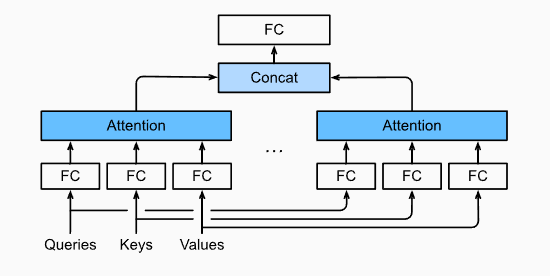
\includegraphics[width=\linewidth]{Figures/background/Multihead.png}
    \caption{Multi-head attention, where multiple heads are concatenated then linearly transformed, (\cite{goodfellow2016dive})}
    \label{fig:attention}
\end{figure}



Given a query $\mathbf{q} \in \mathbb{R}^{d_{q}}$, a key $\mathbf{k_{i}} \in \mathbb{R}^{d_{k}}$ and a value $\mathbf{v_{i}} \in \mathbb{R}^{d_{v}}$, each attention head $h_{i}(i=1,...,h)$ is calculated as:

\begin{equation}
h_{i}=f(\mathbf{W_{i}}^{(q)}\mathbf{q},\mathbf{W_{i}}^{(k)}\mathbf{k_{i}},\mathbf{W_{i}}^{(v)}\mathbf{v_{i}}) \in \mathbb{R}^{p_{v}}
\end{equation}

where $\mathbf{W_{i}}^{(q)} \in \mathbb{R}^{p_{q} \times d_{q}}$, $\mathbf{W_{i}}^{(k)} \in \mathbb{R}^{p_{k} \times d_{k}}$ and $\mathbf{W_{i}}^{(v)} \in \mathbb{R}^{p_{v} \times d_{v}}$ are parameters learnable by the model (\textbf{Backpropagation}) and $f(.)$ is the attention pooling function, where the attention function can be for example the dot product attention function. 

The output of the multihead attention mechanism is calculated as:

\begin{equation}
    \mathbf{W_{o}} \begin{bmatrix}
h_1 \\
h_2 \\
\vdots \\
h_h \\
\end{bmatrix} \in \mathbb{R}^{p_{o}}
\end{equation}

where $\mathbf{W_{o}} \in \mathbb{R}^{p_{o} \times hp_{v}}$ is the parameter learnable by the model (\textbf{Backpropagation}). 
\newpage
\textbf{Self Attention}

Self attention is a mechanism that allows capturing relationships between elements of a sequence (for example, between words in a text) but also between elements of non-sequential data (for example, between pixels in an image). Well, self attention allows finding the attention of each element over all the others. Given an input sequence of $n$ elements $\mathbf{x_{1}},...,\mathbf{x_{n}}$ where $\mathbf{x_{i} \in \mathbb{R}^{d}} (1 \leq i \leq n)$. Then, for every element is calculated $\mathbf{q_{i}} \in \mathbb{R}^{d_{k}}, \mathbf{k{i}} \in \mathbb{R}^{d_{k}}, \mathbf{v_{i}} \in \mathbb{R}^{d_{v}}$:

\begin{equation}
    \mathbf{q_{i}}=\mathbf{x_{i}}\mathbf{W_{Q_{i}}}
\end{equation}

\begin{equation}
    \mathbf{k_{i}}=\mathbf{x_{i}}\mathbf{W_{K_{i}}}
\end{equation}

\begin{equation}
    \mathbf{v_{i}}=\mathbf{x_{i}}\mathbf{W_{V_{i}}}
\end{equation}

where $\mathbf{W_{Q}} \in \mathbb{R}^{d \times d_{k}}$, $\mathbf{W_{K}} \in \mathbb{R}^{d \times d_{k}}$ and $\mathbf{W_{V}} \in \mathbb{R}^{d \times d_{v}}$ are parameters learnable by the model (\textbf{Backpropagation}). After is calculated the attention weights between the element at position $i$ and all other elements:

\begin{equation}
     \alpha (\mathbf{q_{i}},\mathbf{k_{j}})=SOFTMAX(\frac{\mathbf{q_{i}}^{T}\mathbf{k_{j}}}{\sqrt{d}}) \in \mathbb{R}
\end{equation}

as you can see this is calculated using the query of the element at position $i$ and the keys of the other elements. After is calculated the pooling attention of the element at position $i$ over all other elements:

\begin{equation}
    Attention(\mathbf{q_{i}},\mathbf{D_{j}})=\sum_{m} \alpha (\mathbf{q_{i}},\mathbf{k_{j}})\mathbf{v_{j}} \in \mathbb{R}^v
\end{equation}

The same procedure is repeated over all the other elements and with all the other elements.
\newpage
\textbf{Positional Embedding}
\\\\
Before passing the input $\mathbf{X} \in \mathbb{R}^{n \times d}$ through a self-attention mechanism, its respective positional information must be added to each element $\mathbf{x_{i}} \in \mathbb{R}^{d}$; since self-attention is a parallel mechanism, the positional information of the elements is lost. Then positional encoding consists of adding to each element a vector that encodes both positional information and frequency information. This positional coding can be learned by the model (backpropagation) or it can be fixed a priori using sine and cosine functions.
\\\\
If you have some input data $\mathbf{X} \in \mathbb{R}^{n \times d}$, then the output of the positional encoding is $\mathbf{X}+\mathbf{P}$ where $\mathbf{P} \in \mathbb{R}^{n \times d}$  is a positional embedding matrix. Then, the positional embedding for the i-th element in every column(j) of the element is: 

\begin{equation}
    p_{i,2j}=\sin(\frac{i}{10000^{\frac{2j}{d}}}) \in [-1,1]
\end{equation},
\begin{equation}
    p_{i,2j+1}=\cos(\frac{i}{10000^{\frac{2j}{d}}}) \in [-1,1]
\end{equation}

where $p_{i,2j}$ is for pairs columns and $p_{i,2j+1}$ is for uninpairs columns.


\subsection{Transformer Architecture}


As you have seen, self attention allows both parallel computation and long-term relationship coding. So it is attractive to design deep architectures using self-attention, then a transformer is a deep architecture that uses stacked self-attention mechanisms.

\begin{figure}[h!]
    \centering%width=0.7\linewidth
    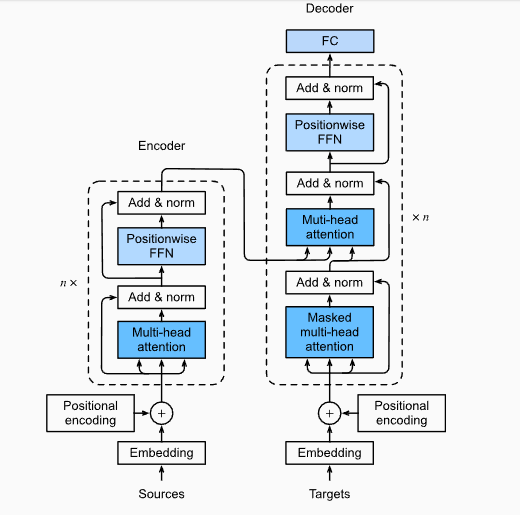
\includegraphics[width=\linewidth]{Figures/background/Transformer.png}
    \caption{Transformer Architecture, (\cite{goodfellow2016dive})}
    \label{fig:attention}
\end{figure}

\newpage
\textbf{Positional Encoding}
\\\\
First, input (source) and output (target) data are passed through a positional encoding before entering the encoder and decoder respectively; since they will enter self attention mechanisms.

\begin{equation}
    \mathbf{X}'=\mathbf{X}+\mathbf{P_{x}  \in \mathbb{R}^{n \times d}}
\end{equation}
\begin{equation}
    \mathbf{Y}'=\mathbf{Y}+\mathbf{P_{y}  \in \mathbb{R}^{n \times d}}
\end{equation}

where $\mathbf{X} \in \mathbb{R}^{n \times d}$ is the input data, $\mathbf{Y} \in \mathbb{R}^{n \times d}$
is the output data and $\mathbf{P_{x}}  \in \mathbb{R}^{n \times d}$, $\mathbf{P_{y}}  \in \mathbb{R}^{n \times d}$ are the respective positional embedding matrices.
\\\\
\textbf{Encoder Tranformer}
\\\\
Encoder transformer is a stack of $n$ identical layers, which have two sub layers: The first is a multi-headed self attention pooling and the second is a positionwise feed-forward network (FFN). The FFN is in charge of introducing non-linearity to the model (using a Relu activation function); as this allows the model to capture characteristics and patterns of each position in the sequence.

\begin{equation}
    FFN(x)=max(0,\mathbf{x}\mathbf{W_{1}}+b_{1})\mathbf{W_{2}}+b_{2}
\end{equation}

Where $x$ is the input to FFN and $\mathbf{W_{1}}, \mathbf{W_{2}},b_{1}, b_{2}$ are the parameters learned by the model (Backpropagation).

A residual connection and a layer normalization are applied to both sublayers. The residual connection consists of adding a direct connection (sum) between the input and output of the sublayer ; as this will allow the original input to be preserved throughout the model and flow unhindered through the model.

\begin{equation}
    \mathbf{Y} = \mathbf{X}+sublayer(\mathbf{X}) \in \mathbb{R}^{n \times d}
\end{equation}

Then the layer normalization is applied after each residual connection, this in order to reduce the variance of the activations and help the gradient to converge faster.
\\\\
\textbf{Decoder Transformer}
\\\\
The decoder is also a stack of $n$ identical layers with residual connections and layer normalizations. But here, each layer has a third sublayer called encoder-decoder attention mechanism or cross attention mechanism, which allows communication between encoder and decoder; as it allows the decoder to service the encoder outputs, allowing the relevant information to flow from the encoder to the decoder. Here the queries are from the output of the previous layer of the decoder and the keys and values are from the output of the encoder. 
\newpage
It is important to note that the large language models used in this research, such as BERT (\cite{devlin2018bert}), Distilbert (\cite{sanh2019distilbert}) and Roberta (\cite{liu2019roberta}), are models with encoder-only architectures; since in this research we have worked on the task of extractive question answering, which is a task that is merely extractive, but not generative.